\subsection{PIT Histograms}
\label{sec:pit-histogram-explanation}

PIT histograms are an important tool for evaluating probabilistic calibration of a forecast. 
Let \(F\) denote a CDF for an observation \(Y\). The probability integral 
transform (PIT) of \(F\) is the random variable \(Z_F = F(Y-) + V(F(Y) - F(Y-))\) 
where \(V \sim U(0,1)\). 
The probabiliy integral transform is the value that the predictive CDF 
attains at the observation \(Y\). \Textcite{Rueschendorf2009} shows that if \(Y \sim F\), \(Z_F\) is standard uniformly distributed.

\Textcite{Gneiting2014} define the different dispersion types as follows:
The PIT is used to evaluate the probabilistic calibration of a forecast. 
A forecast \(F\) is probabilistically calibrated if its PIT \(Z_F\) 
is uniformly distributed on the unit interval. 
It is called overdispersed if \(\mathrm{var}(Z_F) < \frac{1}{12}\) or if 
the PIT histogram has a \(\cap\)-shape. We get underdispersion if 
\(\mathrm{var}(Z_F) > \frac{1}{12}\) or if the PIT histogram has a \(\cup\)-shape. 
A forecast is neutrally dispersed if \(\mathrm{var}(Z_F) = \frac{1}{12}\).
Overdispersion indicate a too high estimated variance and underdispersion indicate 
that the variance of the forecast is too low. 
Figure \ref{fig:dispersion} shows a PIT with \(\mathrm{var}(Z_F) < \frac{1}{12}\), 
\(\mathrm{var}(Z_F) = \frac{1}{12}\) as well as a PIT with \(\mathrm{var}(Z_F) > \frac{1}{12}\), 
i.e., an overdispersed, a probabilistically calibrated and therefore neutrally dispersed as well as an underdispersed forecast.

\begin{figure}[h]%
    \centering
    \subfloat[\centering Overdispersed]{{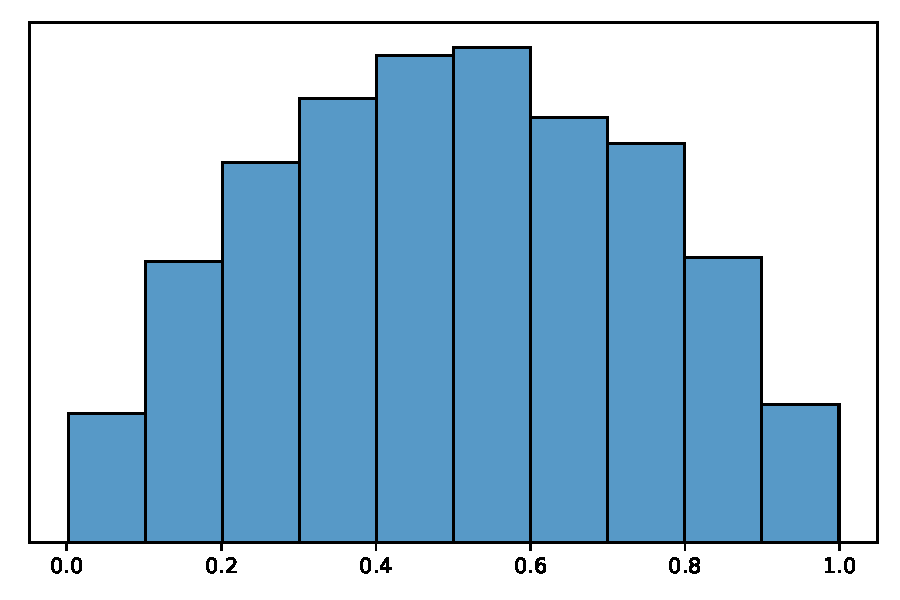
\includegraphics[width=0.3\textwidth]{plots/pit/overdispersed.pdf} \label{fig:pit-overdispersed} }}
    \subfloat[\centering Neturally dispersed]{{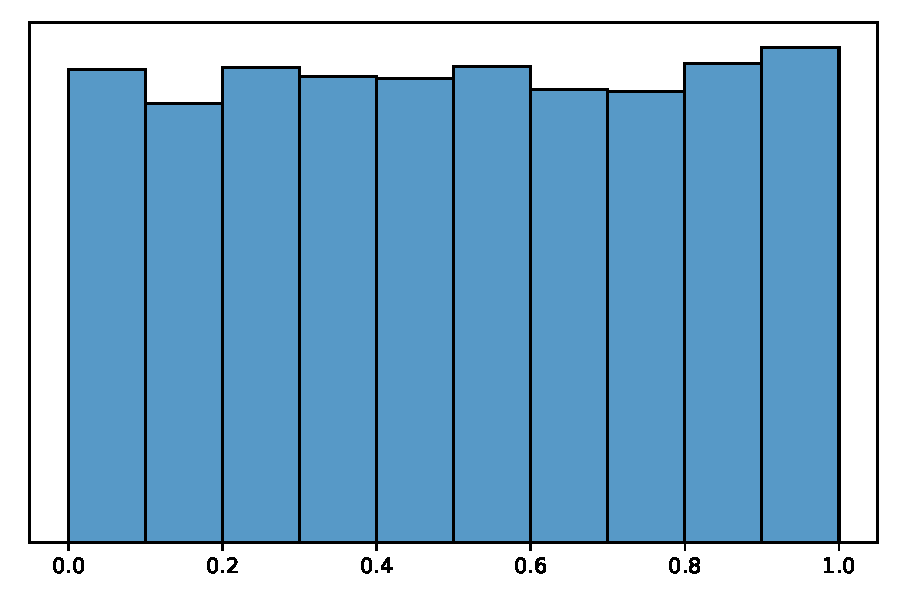
\includegraphics[width=0.3\textwidth]{plots/pit/neutrally_dispersed.pdf} \label{fig:pit-neutrally-dispersed} }}
    \subfloat[\centering Underdispersed]{{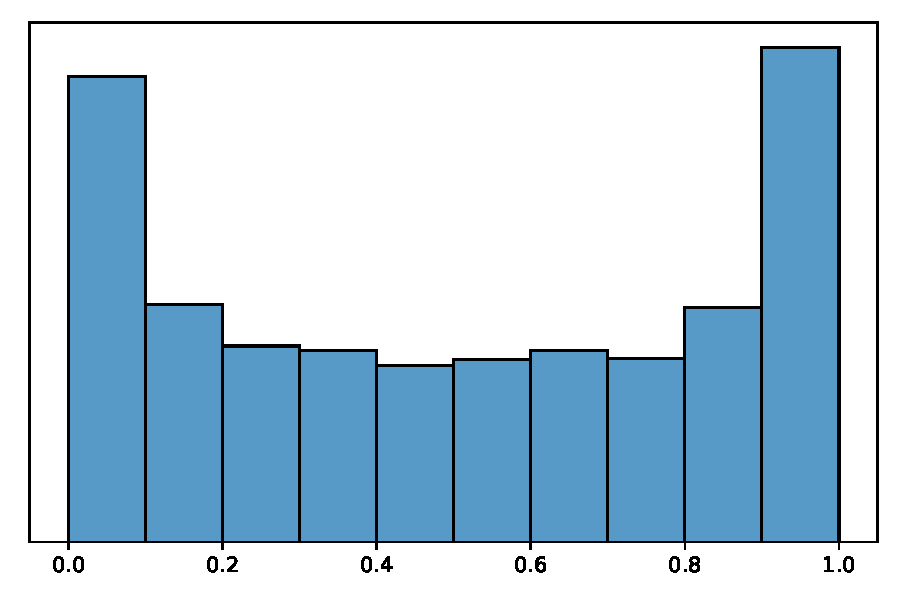
\includegraphics[width=0.3\textwidth]{plots/pit/underdispersed.pdf} \label{fig:pit-underdispersed} }}
    \caption[Dispersion types for PITs]{Dispersion types for PITs. The PIT of an overdispersed forecast is formed like a \(\cap\) (Figure \ref{fig:pit-overdispersed}). 
    Figure \ref{fig:pit-neutrally-dispersed} is probabilistically calibrated, i.e. \(Z_F \sim U(0,1)\), and therefore neutrally dispersed. 
    An underdispersed forecast has a PIT that looks like a \(\cup\) (Figure \ref{fig:pit-underdispersed}).}%
    \label{fig:dispersion}%
\end{figure}